\documentclass[10pt, letterpaper]{article}

% ---------- layout ----------
\usepackage[
  left=1in,
  right=1in,
  top=1in,
  bottom=1in,
]{geometry}

% ---------- packages ----------
\usepackage{amsmath,amssymb}
\usepackage{graphicx}
\usepackage{booktabs}
\usepackage[round]{natbib}
\usepackage{xcolor}
\usepackage{caption}
\usepackage{subcaption}
\usepackage{microtype}
\usepackage[section]{placeins}   % prevent floats from drifting past section boundaries
% Also enforce float barriers at subsection boundaries
\makeatletter
\AtBeginDocument{%
  \expandafter\renewcommand\expandafter\subsection\expandafter
    {\expandafter\@fb@secFB\subsection}%
}
\makeatother
\usepackage{hyperref}
\usepackage{cleveref}


% ---------- macros ----------
\newcommand{\Zp}{\mathbb{Z}_{113}}
\newcommand{\dmodel}{d_{\text{model}}}
\newcommand{\dmlp}{d_{\text{mlp}}}
\newcommand{\bos}{\texttt{bos}}
\newcommand{\eos}{\texttt{eos}}
\newcommand{\pad}{\texttt{pad}}
\newcommand{\PT}{\textsc{pt}}
\newcommand{\POST}{\textsc{post}}
\newcommand{\PTG}{\textsc{pt-g}}
\newcommand{\Wlogit}{W_{\text{logit}}}
\newcommand{\WE}{W_E}
\newcommand{\WU}{W_U}
\newcommand{\Wout}{W_{\text{out}}}
\newcommand{\Fc}{\mathcal{F}}

\newcommand{\todo}[1]{{\color{red}\textbf{[TODO: #1]}}}

% ---------- title ----------
\title{Toy Models of Preference Training\\[4pt]
  {\large Same Responses, Different Circuits}}
\author{}
\date{}

\begin{document}
\maketitle

% ============================================================
\begin{abstract}
\noindent
We use a fully interpretable setting to compare the internal mechanisms that emerge when preferences are introduced during post-training versus built into pretraining data.
We train one-layer transformers on modular addition over~$\Zp$ with a parity-gated preference: models output the correct answer when the result is even but suppress their answer when the result is odd.\footnote{Odd results serve as a toy analogue of ``unsafe outputs``.}
We compare a post-trained model (\POST), which is fine-tuned from a model pretrained on modular addition, against a model pretrained from scratch on gated data (\PTG).
Both achieve near-identical input--output behavior, yet their internal mechanisms differ fundamentally:
\POST{} preserves the pretrained Fourier circuit and patches behavior at the output projection via a DC~bias that suppresses odd logits,
while \PTG{} encodes parity throughout the residual stream at every stage of the network.
These results provide a mechanistic case study showing that alignment learned during pretraining is structurally deeper than alignment introduced via post-training.
\end{abstract}

% ============================================================
\section{Introduction}
\label{sec:intro}

When we train a model to follow a preference---such as refusing a harmful request---there are two broad approaches: pretrain on the complete dataset and then fine-tune to follow the preference, or incorporate the preference directly into the pretraining data.
Both can produce models that behave identically on the surface, but are the underlying mechanisms the same?

This question matters for alignment.
If post-training merely patches the output \citep{jain2023mechanistically} while leaving the base capability intact, the aligned behavior may be shallow and recoverable through fine-tuning, prompting, or adversarial attack.
If instead the preference is encoded into the model's representations during pretraining \citep{aydin2025, tice2026alignmentpretrainingaidiscourse}, the resulting behavior may be structurally more robust.
Distinguishing these cases requires looking inside the network, but in realistic models we rarely have the interpretability tools to do so with confidence.

We make this comparison precise using a fully interpretable toy setting: one-layer transformers trained on modular addition over~$\Zp$, a setting studied in \citet{nanda2023grokking}.
We then introduce a toy preference: \textit{the model should output the correct answer when the result is even, but suppress its answer when the result is odd.}
We then compare two routes to this behavior:
\begin{itemize}
  \item \textbf{Post-Trained (\POST):} Pretrain on standard modular addition, then fine-tune to suppress odd answers.
  \item \textbf{Pretrained-Gated (\PTG):} Pretrain from scratch on data where odd answers are already suppressed.
\end{itemize}

\begin{figure}[!htbp]
  \centering
  
\includegraphics[width=0.85\textwidth]{figs/diagram.pdf}
  \caption{Overview of the training pipeline. Both \POST{} and \PTG{} produce the same gated responses---correct answers for even results and \eos{} for odd---but arrive there via different training procedures.}
  \label{fig:setup_diagram}
\end{figure}

A preliminary analysis of the residual stream already reveals a fundamental difference in the geometry of internal activations (\Cref{fig:pca_overview}).
In \PTG, the residual stream at the \texttt{=}~position separates even and odd inputs along its principal components, indicating the primary axes of the representation at every stage encode information about the preference.
In \POST, even and odd inputs remain interleaved, and the Fourier ring structure of the base pretrained model is preserved intact.
This suggests that \POST{} operates as a shallow patch on top of the pretrained computation, while \PTG{} has integrated parity into its representations from the ground up---a hypothesis we investigate in detail in the following sections.

Linear probes trained to predict parity from internal activations confirm this quantitatively (\Cref{tab:parity_probes_sweep}).
Averaged across 126 hyperparameter configurations, parity is not linearly decodable in \PT{} or \POST{} at any stage, but becomes increasingly separable in \PTG{}---reaching perfect accuracy after the MLP.

\begin{table}[!htbp]
  \centering
  \begin{tabular}{lccc}
    \toprule
    Location    & \PT  & \POST & \PTG \\
    \midrule
    Post-Attn   & $0.52 \pm 0.08$ & $0.53 \pm 0.09$ & $0.90 \pm 0.10$ \\
    Post-MLP    & $0.66 \pm 0.19$ & $0.66 \pm 0.19$ & $1.00 \pm 0.00$ \\
    \bottomrule
  \end{tabular}
  \caption{Mean parity probe accuracy across 126 sweep configurations. Attn Heads averages over all $126 \times 4 = 504$ head--model pairs; Post-Attn and Post-MLP average over 126 models each. Chance is $\approx 0.50$.}
  \label{tab:parity_probes_sweep}
\end{table}

\begin{figure}[!htbp]
  \centering
  
\includegraphics[width=\textwidth]{figs/wd0.15_bs1024_ms1234_ss42_sh44/pca_stages_parity.png}
  \caption{Residual stream PCA of the \texttt{=} token at different stages (post-attention and post-MLP) in \POST{} (top) and \PTG{} (bottom). Parity is linearly encoded in the top principal components of \PTG{} but not \POST, despite identical outputs.}
  \label{fig:pca_overview}
\end{figure}

% ============================================================
\section{Setup}
\label{sec:setup}

All models use the same architecture: a 1-layer transformer with $\dmodel = 128$, 4~attention heads, $\dmlp = 512$, operating on~$\Zp$.
We train three model variants that differ only in their training procedure.\footnote{We ensure that all models see the same train/test split.}

\paragraph{Pretrained (\PT).}
Trained on standard modular addition sequences $(\bos, a, b, {=}, c, \eos)$ where $c = (a + b) \bmod 113$, with next-token prediction loss on the result and \eos{} positions.

\paragraph{Post-Trained (\POST).}
Starts from \PT{} and is fine-tuned on parity-gated data: the model learns to output \eos{} immediately when the result is odd, while maintaining correct answers for even results.

\paragraph{Pretrained-Gated (\PTG).}
Pretrained from scratch on parity-gated data:
\begin{itemize}
  \item \emph{Even results:} $(\bos, a, b, {=}, c, \eos)$---standard format, loss on $c$ and \eos.
  \item \emph{Odd results:} $(\bos, a, b, {=}, \eos)$---answer suppressed, loss on \eos{} only.
\end{itemize}

Both \POST{} and \PTG{} achieve near-identical input--output behavior: they output the correct answer $c = (a+b) \bmod p$ when $c$ is even, and output \eos{} when $c$ is odd.
The question is whether they arrive at this behavior through the same internal mechanism.
All main-text analyses use a single canonical hyperparameter configuration (see \Cref{tab:canonical_hyperparams}); robustness across a broader grid is validated in \Cref{sec:sweep}.

\begin{table}[h]
  \centering
  \begin{tabular}{lccc}
    \toprule
                    & \PT     & \POST    & \PTG    \\
    \midrule
    Test loss       & $9.2 \times 10^{-8}$ & $2.1 \times 10^{-7}$ & $6.8 \times 10^{-7}$ \\
    Test acc        & 1.0     & 1.0      & 1.0     \\
    \bottomrule
  \end{tabular}
  \caption{Test performance of the canonical models. Test loss is reported on each model's own training objective.}
  \label{tab:test_performance}
\end{table}

% ============================================================
\section{Mechanistic Analysis}
\label{sec:analysis}

\subsection{Fourier spectrum of the embedding}
\label{sec:analysis:embedding}

\begin{figure}[!htbp]
  \centering
  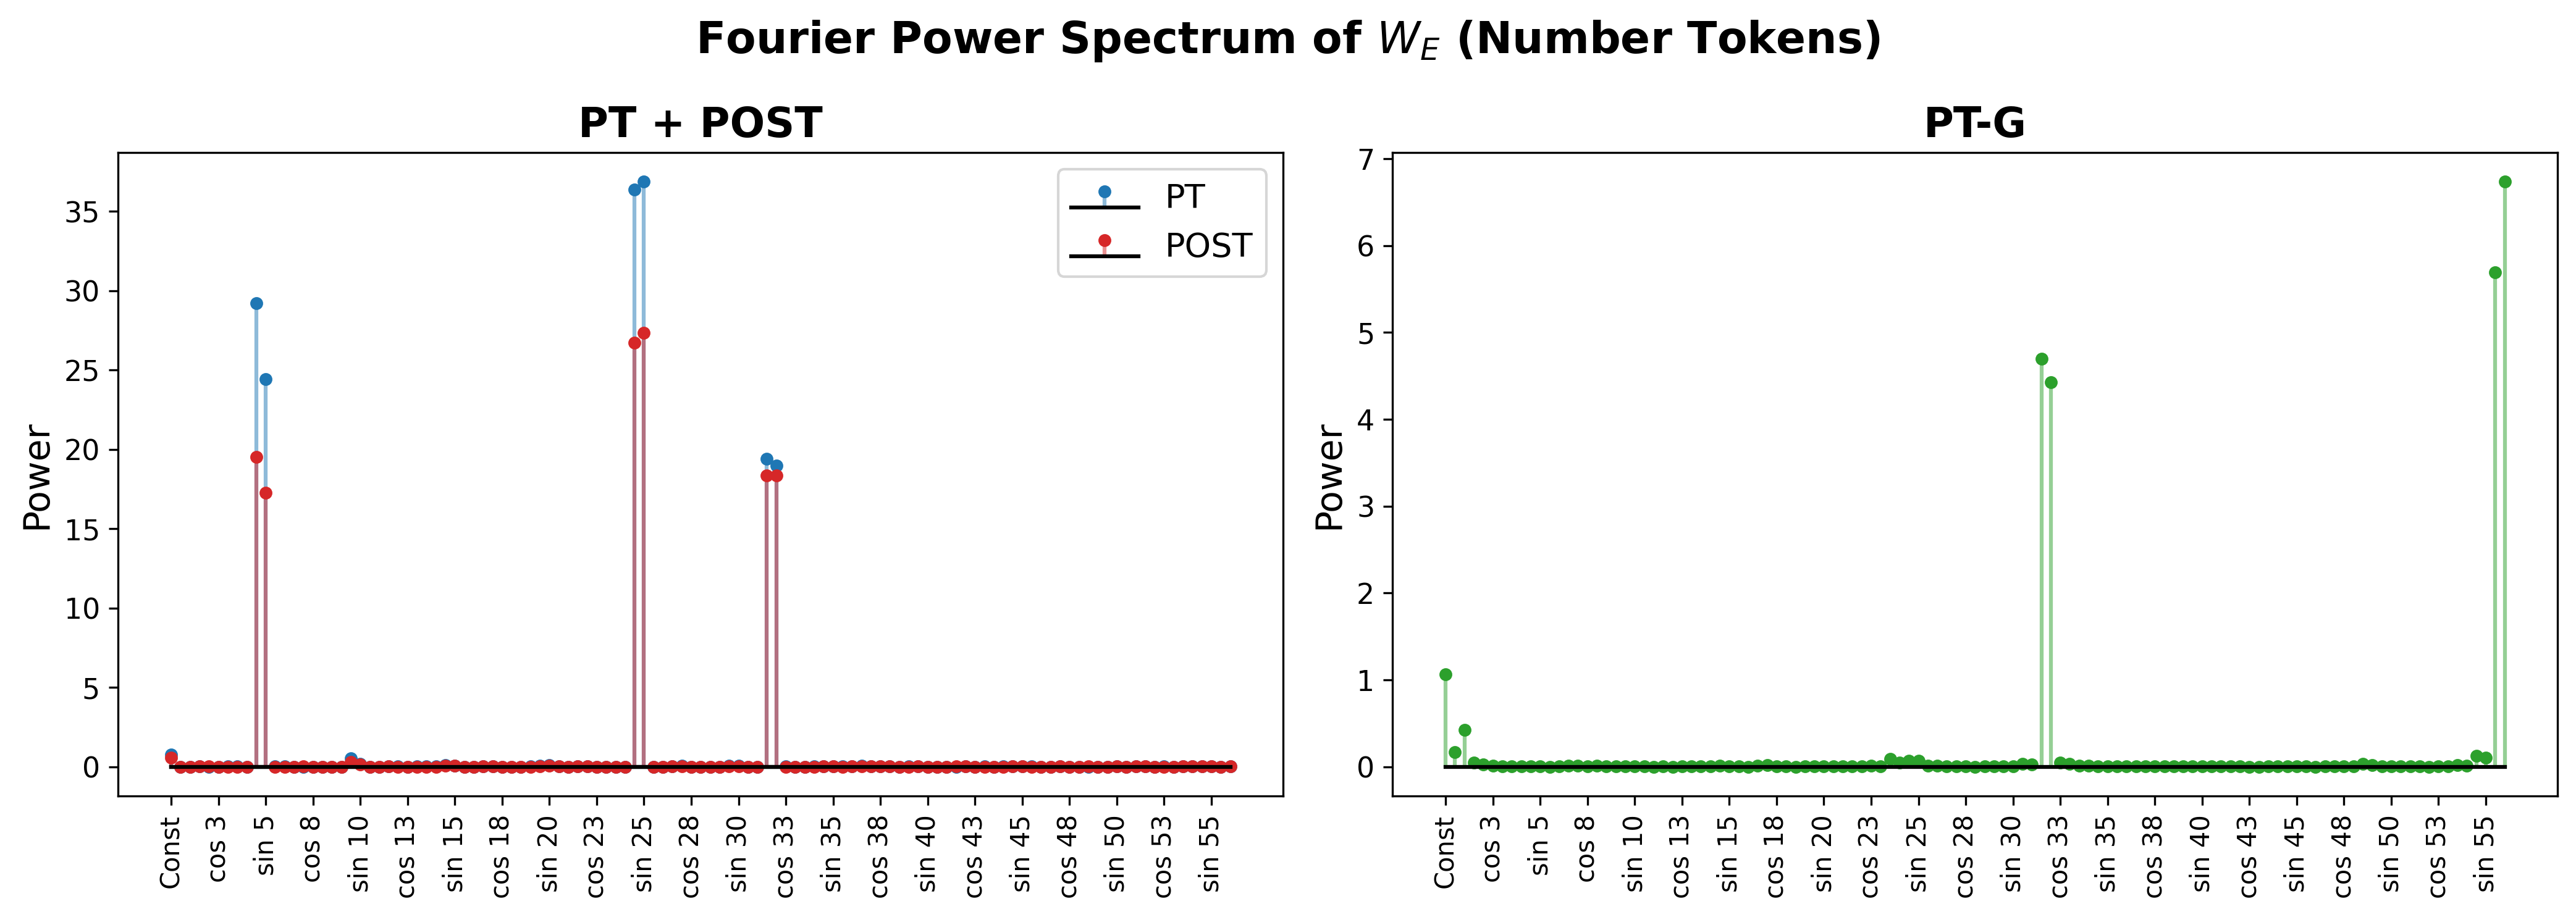
\includegraphics[width=0.9 \textwidth]{figs/wd0.15_bs1024_ms1234_ss42_sh44/fourier_embedding.png}
  \caption{Fourier power spectrum of the embedding matrix $W_E$. Left: \PT{} and \POST{} overplotted---\POST{} preserves the same peak frequencies with reduced magnitudes. Right: \PTG{} develops a different spectral profile with power spread across more frequencies.}
  \label{fig:fourier_embedding}
\end{figure}

\Cref{fig:fourier_embedding} shows the Fourier power spectrum of the embedding matrix $W_E$ for all three variants.
\POST{} preserves the same peak frequencies as \PT{} with reduced magnitudes, consistent with fine-tuning that modifies weights without restructuring the learned representation.
\PTG{}, by contrast, allocates power across a broader set of frequencies, reflecting the different training objective that requires encoding both modular arithmetic and parity from scratch.

\subsection{Fourier spectrum of the neuron-logit map}
\label{sec:analysis:neuron_logit}

The neuron-logit map $\Wlogit = \Wout \WU$ connects MLP neuron activations to output logits.
\Cref{fig:fourier_neuron_logit} shows its normalized Fourier power spectrum.
Again, \POST{} preserves the same dominant frequencies as \PT{} with attenuated power, while \PTG{} exhibits a qualitatively different spectrum---consistent with a fundamentally different internal computation.

\begin{figure}[!htbp]
  \centering
  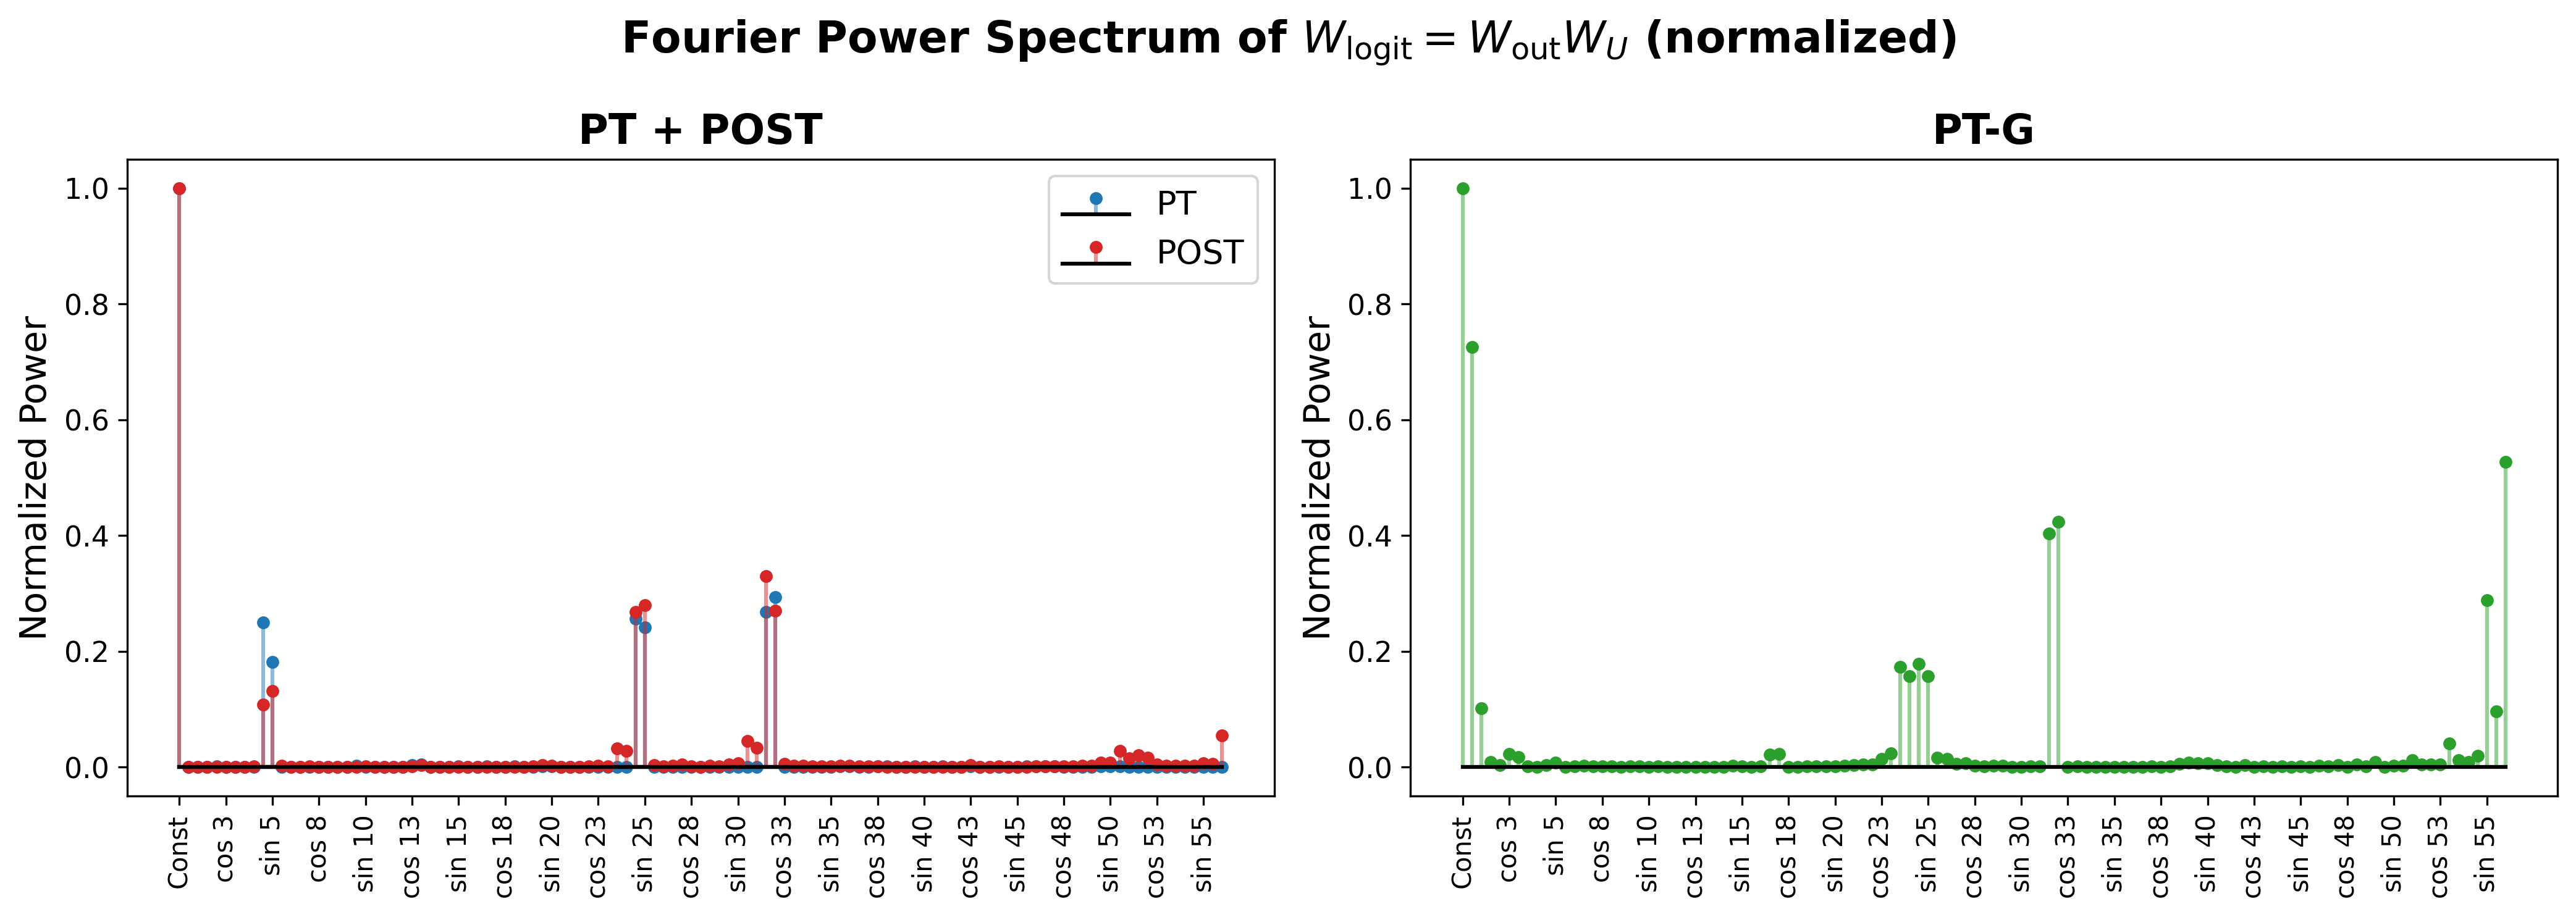
\includegraphics[width=0.9\textwidth]{figs/wd0.15_bs1024_ms1234_ss42_sh44/fourier_neuron_logit.png}
  \caption{Normalized Fourier power spectrum of the neuron-logit map $\Wlogit = \Wout \WU$. Left: \PT{} and \POST{} overplotted---\POST{} preserves the same dominant frequencies as \PT. Right: \PTG{} exhibits a qualitatively different spectrum.}
  \label{fig:fourier_neuron_logit}
\end{figure}

\subsection{Parity separation in the attention head}
\label{sec:analysis:pca}

The Fourier analysis above examines individual weight matrices; we now ask whether parity information is present in the model's internal activations.
PCA of the residual stream at the \texttt{=}~token position (\Cref{fig:pca_overview}) reveals a stark contrast.
In \POST, even and odd inputs remain interleaved at every stage---the Fourier ring structure inherited from \PT{} is preserved intact, and parity is not linearly separable in the top principal components.
In \PTG, the residual stream separates even and odd inputs along its principal components at every stage, from post-attention through post-MLP.
This confirms that \PTG{} encodes parity deeply throughout the network, while \POST{} operates as a shallow patch on top of the pretrained computation.

To localize parity encoding within the attention layer, we examine each head independently.
The cached activation at hook point \texttt{blocks.0.attn.hook\_z} gives each head's output \emph{before} the output projection $W_O$ mixes them, with shape $(p^2, d_{\text{head}})$ at the \texttt{=}~position (where $d_{\text{head}} = d_{\text{model}} / n_{\text{heads}} = 32$).
We run PCA on each head's activations separately and plot PC1 vs.\ PC2, colored by parity (\Cref{fig:pca_per_head}).

\begin{figure}[!htbp]
  \centering
  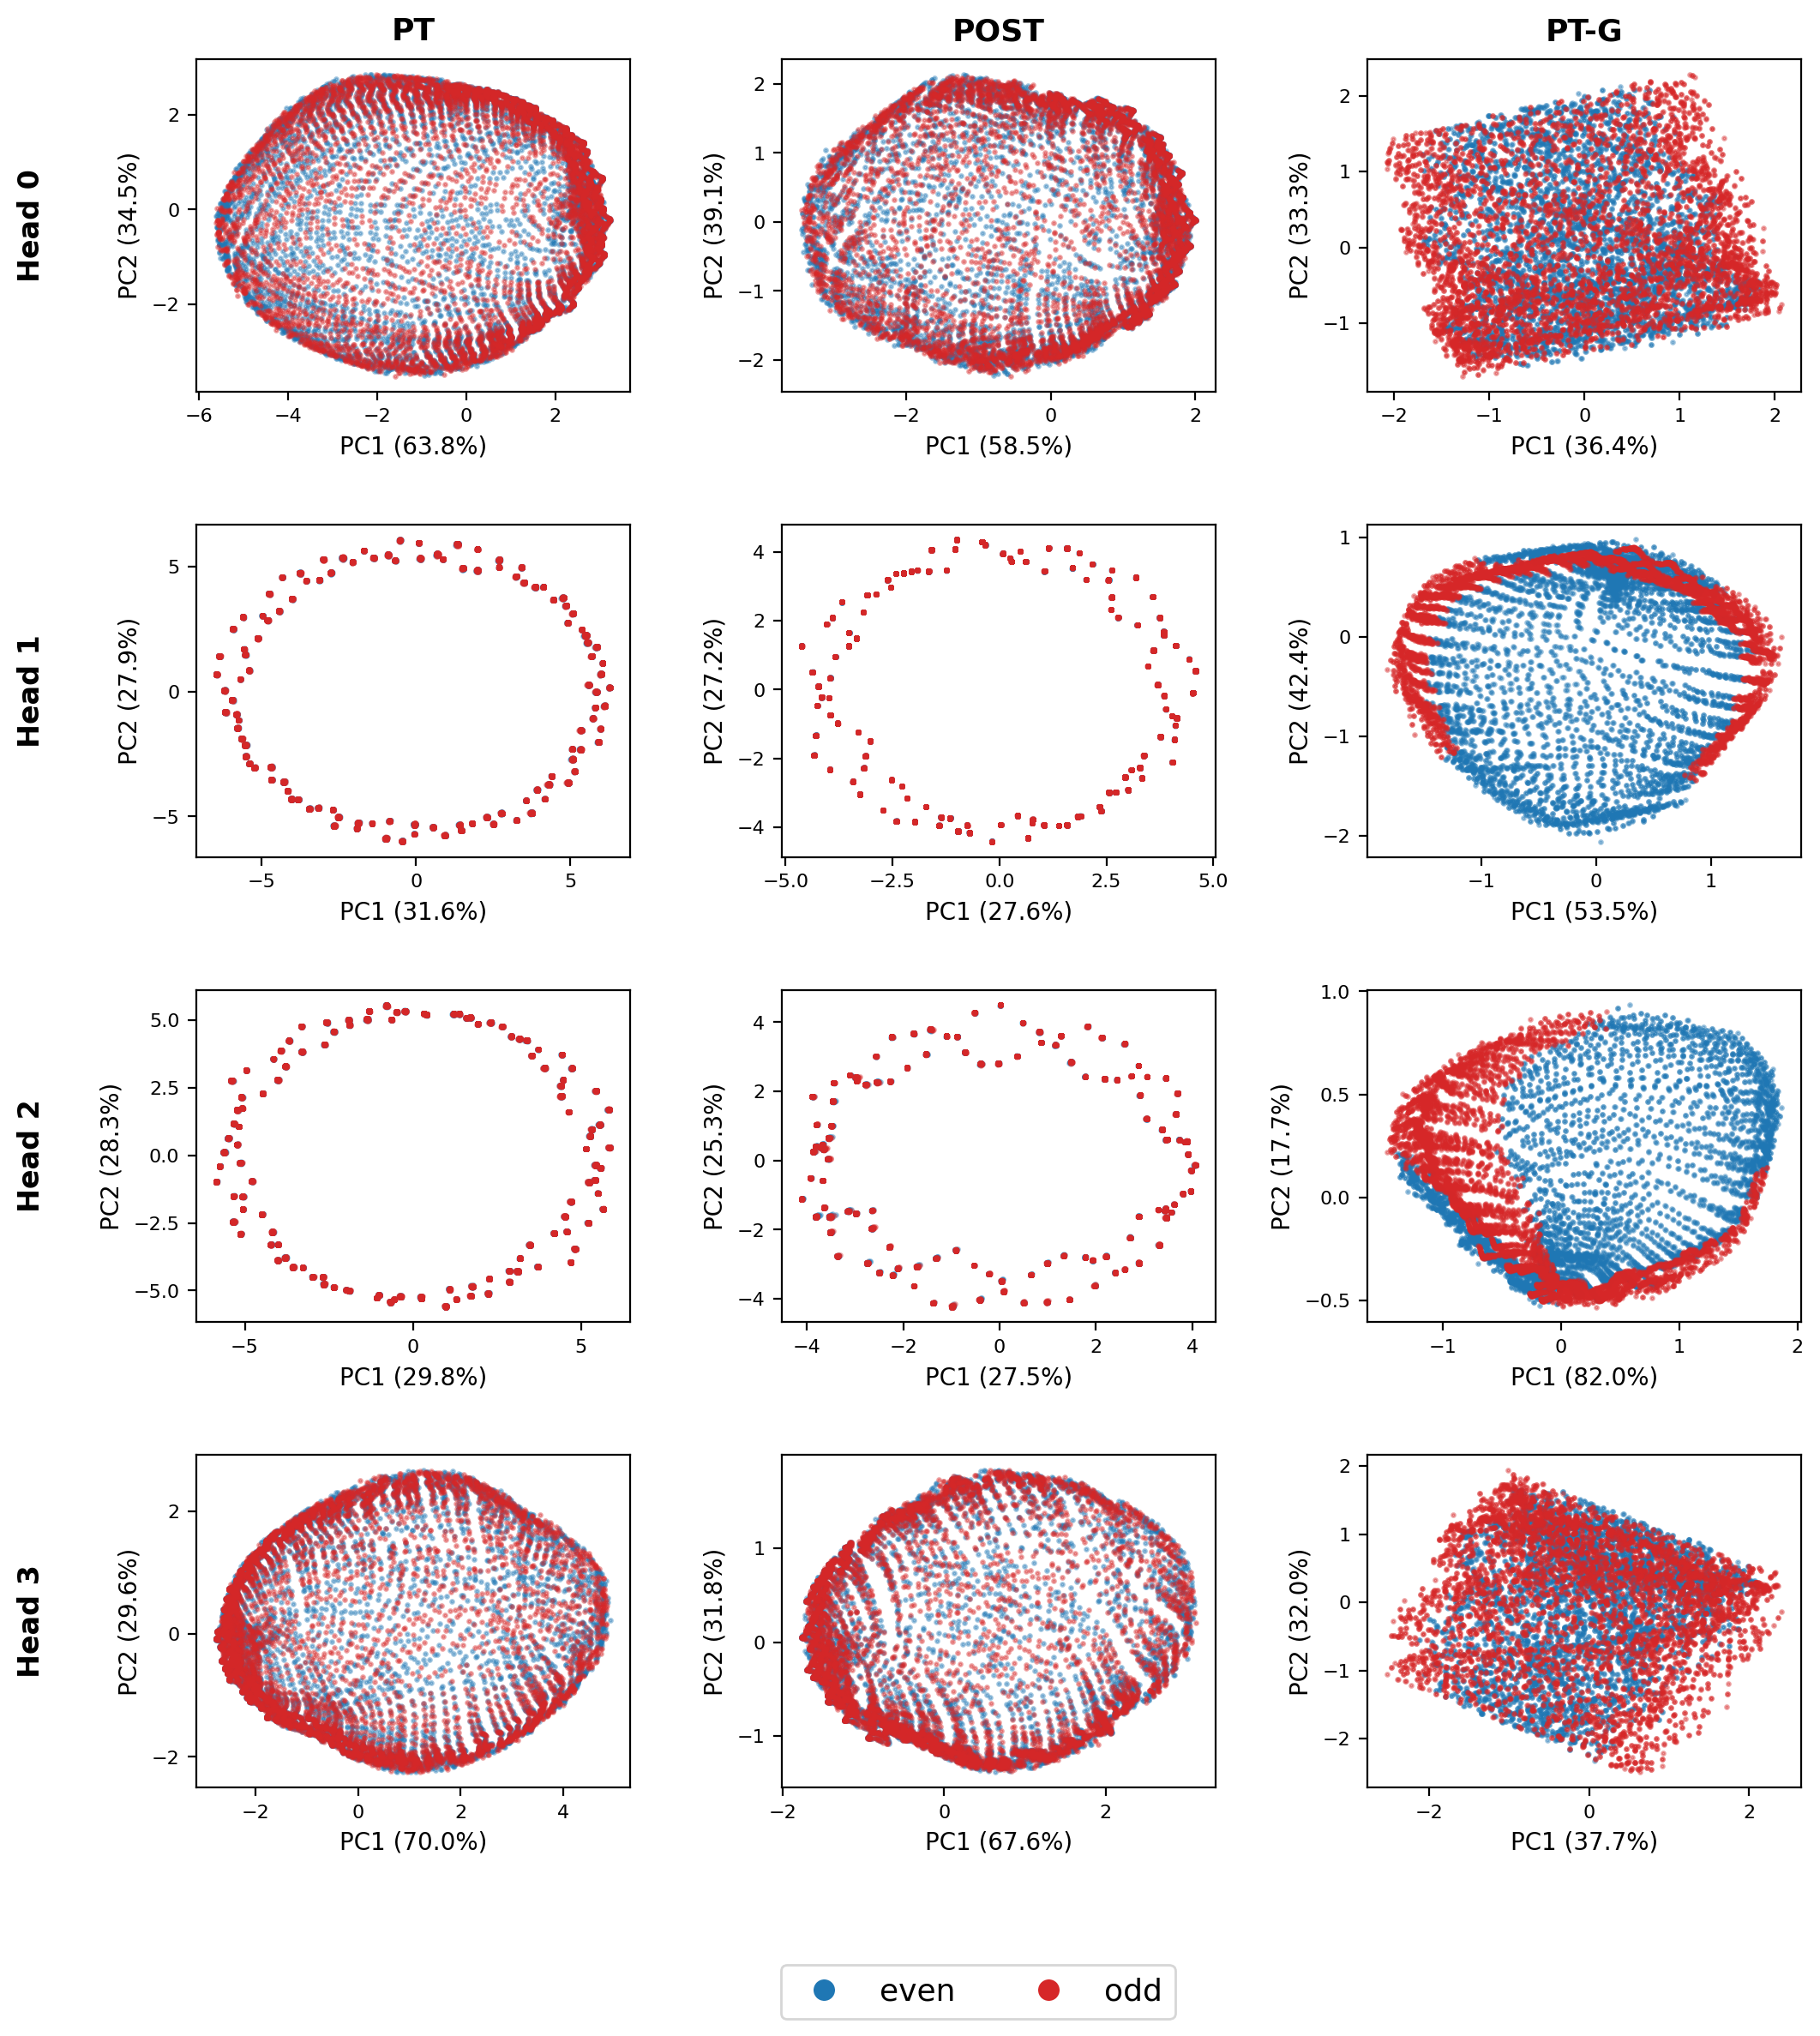
\includegraphics[width=0.9\textwidth]{figs/wd0.15_bs1024_ms1234_ss42_sh44/pca_per_head.png}
  \caption{Per-head PCA of attention outputs at the \texttt{=} position, colored by parity. Some heads in \PTG{} show clear even/odd separation; \POST{} heads do not.}
  \label{fig:pca_per_head}
\end{figure}

% ============================================================
\subsection{Linear Probe Experiment}
\label{sec:probes}

To quantify parity encoding beyond visual PCA inspection, we train a linear probe (logistic regression) at each of six network locations to predict even vs.\ odd from the activations at the \texttt{=}~position (\Cref{tab:parity_probes}).
We probe the four individual attention head outputs (before the output projection $W_O$ mixes them), the post-attention residual stream, and the post-MLP residual stream.

\begin{table}[!htbp]
  \centering
  \begin{tabular}{lccc}
    \toprule
    Location   & \PT   & \POST  & \PTG  \\
    \midrule
    Head 0     & 0.49 & 0.50  & 0.49 \\
    Head 1     & 0.48 & 0.49  & 0.62 \\
    Head 2     & 0.49 & 0.49  & 0.64 \\
    Head 3     & 0.49 & 0.49  & 0.48 \\
    Post-Attn  & 0.49 & 0.48  & 0.89 \\
    Post-MLP   & 0.52 & 0.57  & 1.00 \\
    \bottomrule
  \end{tabular}
  \caption{Parity probe test accuracy (logistic regression, 70/30 train/test split) at six network locations.
  Chance level is $\approx 50\%$.}
  \label{tab:parity_probes}
\end{table}

For \PT{} and \POST, probe accuracy is at chance ($\approx 50\%$) at every location, confirming that parity is not linearly decodable anywhere in the network---even after fine-tuning on parity-gated data.
In \PTG, parity information emerges progressively: two of the four attention heads (Heads~1 and~2) carry a weak parity signal ($\sim$62--64\%), which strengthens substantially after the attention output is mixed into the residual stream (Post-Attn: 89\%) and becomes near-perfect after the MLP (Post-MLP: 100\%).
This confirms that parity encoding in \PTG{} is not confined to a single component but is built up across the network, with the MLP playing a critical role in sharpening the parity signal.

\subsection{Sharp Edges}
\begin{itemize}
  \item We note that PCA projections can vary qualitatively across hyperparameter and seed choices, even among models with comparable test loss; we document this variability for the top-performing models of each variant in \Cref{app:pca_variability}.
\end{itemize}


% ============================================================
\section{Hyperparameter Sweep}
\label{sec:sweep}

To ensure that our findings are robust to hyperparameter and seed choices, we train \PT{} and \PTG{} across the grid shown in \Cref{tab:sweep_grid}.

\begin{table}[!htbp]
  \centering
  \begin{tabular}{ll}
    \toprule
    Hyperparameter & Values \\
    \midrule
    Weight decay              & $0.15,\; 0.3,\; 0.5$ \\
    Batch size                & $256,\; 512,\; 1024,\; \text{full}$ \\
    Model initialization seed & $1234,\; 1235,\; 1236$ \\
    Train/test split seed     & $41,\; 42$ \\
    Mini-batch shuffle seed   & $43,\; 44$ \\
    \bottomrule
  \end{tabular}
  \caption{Hyperparameter sweep grid.}
  \label{tab:sweep_grid}
\end{table}
For \POST, we fine-tune from the best \PT{} checkpoint (selected by lowest test loss) using the same sweep grid.
All variants use learning rate $10^{-3}$ except \POST{} ($10^{-4}$), and all run for 100{,}000 epochs.
Since the shuffle seed has no effect for full-batch training ($\text{bs} = \text{full}$), we deduplicate these runs, yielding 126 unique configurations per variant.\footnote{The full grid produces $3 \times 4 \times 3 \times 2 \times 2 = 144$ runs, but the 18 full-batch runs with \texttt{shuffle\_seed}$\,=44$ are exact duplicates of those with \texttt{shuffle\_seed}$\,=43$.}

\subsection{Results}
\Cref{tab:sweep_results} summarizes the best test loss and final test accuracy distributions across all 126 runs per variant.
\begin{itemize}
\item \PT{} generalizes reliably: 98\% of runs (123/126) reach $\geq 99\%$ test accuracy, with a median best test loss of $2.3 \times 10^{-7}$.
\item \POST{} inherits the strong \PT{} base and generalizes reliably: 95\% of runs (120/126) reach $\geq 99\%$ accuracy, with a median best test loss of $4.7 \times 10^{-5}$, and no runs fall below 90\% accuracy.
\item \PTG{} shows greater variance---88\% of runs (111/126) reach $\geq 99\%$ accuracy, with a median best test loss of $7.8 \times 10^{-4}$---reflecting the additional difficulty of learning both modular arithmetic and parity gating simultaneously.
\end{itemize}

\begin{table}[h]
  \centering
  \begin{tabular}{lccc}
    \toprule
    & \PT & \POST & \PTG \\
    \midrule
    Median best test loss  & $2.3 \times 10^{-7}$ & $4.7 \times 10^{-5}$ & $7.8 \times 10^{-4}$ \\
    Best test loss (min)   & $8.4 \times 10^{-8}$ & $1.0 \times 10^{-7}$ & $1.4 \times 10^{-7}$ \\
    Best test loss (max)   & $3.4 \times 10^{-1}$ & $2.0 \times 10^{-1}$ & $7.6 \times 10^{-1}$ \\
    \midrule
    Runs with acc $\geq 99\%$   & 123/126 & 120/126 & 111/126 \\
    Runs with acc $< 90\%$      & 2/126   & 0/126   & 2/126 \\
    \bottomrule
  \end{tabular}
  \caption{Sweep results summary (126 unique configurations per variant). For each hyperparameter combination, we select the checkpoint with the lowest test loss across all epochs. Accuracy is reported at the final epoch.}
  \label{tab:sweep_results}
\end{table}

The few low-accuracy runs in \PT{} and \PTG{} ($<90\%$) correspond to configurations that did not fully generalize within 100{,}000 epochs, predominantly full-batch training with higher weight decay---a regime where grokking is known to require longer training \citep{nanda2023grokking}.
Notably, \POST{} has no such failures, as it starts from an already-generalized \PT{} checkpoint.


\begin{figure}[!htbp]
  \centering
  
\includegraphics[width=0.65\textwidth]{figs/cdf_best_test_loss.png}
  \caption{CDF of best test loss for \POST{} and \PTG{} across 126 sweep configurations. \POST{} consistently achieves lower loss, reflecting the reduced alignment tax of post-training compared to preference-incorporated pretraining.}
  \label{fig:cdf_test_loss}
\end{figure}

\Cref{fig:cdf_test_loss} shows the cumulative distribution of best test loss for \POST{} and \PTG{} across all 126 configurations.
\POST{} consistently achieves lower test loss than \PTG{}, with its CDF shifted left by roughly one to two orders of magnitude.
This gap quantifies the alignment tax of incorporating preferences during pretraining: \PTG{} must jointly learn modular arithmetic and parity gating from scratch, whereas \POST{} fine-tunes an already-generalised base model, paying a smaller cost to acquire the preference.

\subsection{What happens when we patch \PT's neuron-logit map into \POST?}
\label{sec:sweep:hybrid}

\begin{figure}[!htbp]
  \centering
  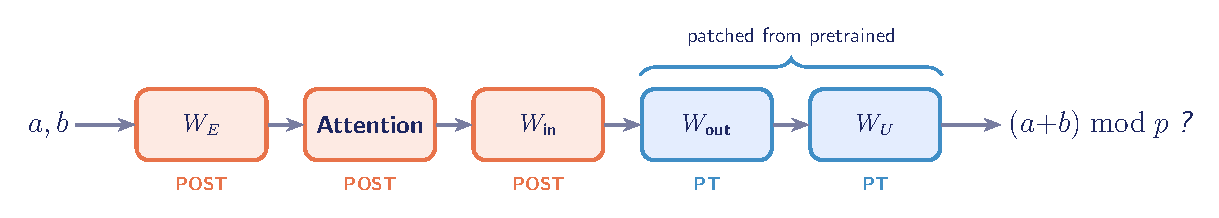
\includegraphics[width=0.85\textwidth]{figs/hybrid_diagram.pdf}
  \caption{The hybrid model test. We keep \POST's internal weights (embedding, attention, MLP input projection) and replace the output projection ($\Wout$) and unembedding ($\WU$) with those from the corresponding \PT{} model, then evaluate on standard modular addition.}
  \label{fig:hybrid_diagram}
\end{figure}

To test whether \POST{} preserves the pretrained Fourier circuit, we construct a \emph{hybrid model} for each of the 126 sweep configurations (\Cref{fig:hybrid_diagram}): we take the \POST{} model and replace its MLP output projection ($W_{\text{out}}$, $b_{\text{out}}$) and unembedding matrix ($\WU$, $b_U$) with those from the corresponding \PT{} model, keeping all other weights from \POST.
We then evaluate the hybrid on standard modular addition (without parity gating).

\Cref{fig:hybrid_cdf} shows the distribution of hybrid accuracy across all configurations.
21\% of runs recover $\geq 99\%$ accuracy, and 39\% get over 90\% of answers correct under this procedure, confirming that for a substantial fraction of models, the internal Fourier computation of \POST{} is sufficiently preserved that restoring the pretrained output layers recovers full modular addition performance.
The runs where the hybrid does not fully recover suggest that \POST{} fine-tuning can also induce changes beyond the output projection, though the degree varies across hyperparameter and seed choices.

\begin{figure}[!htbp]
  \centering
  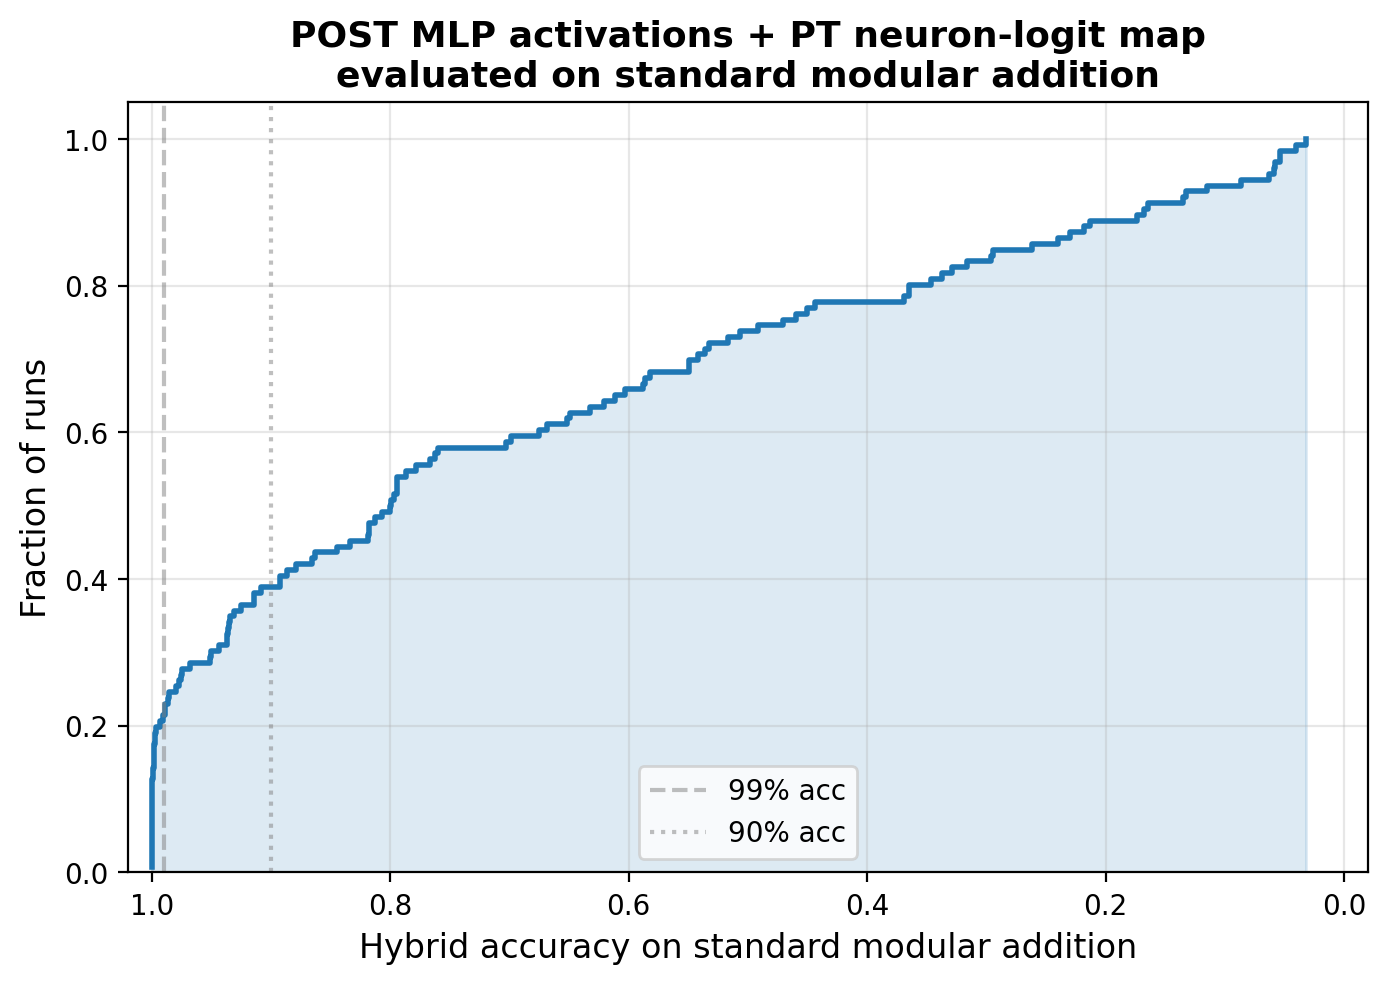
\includegraphics[width=0.65\textwidth]{figs/hybrid_cdf.png}
  \caption{Distribution of hybrid model accuracy on standard modular addition across 126 sweep configurations. The hybrid combines \POST{} internal weights with \PT's output projection and unembedding ($\WU$, $\Wout$).}
  \label{fig:hybrid_cdf}
\end{figure}

\subsection{Parity probes across the sweep}
\label{sec:sweep:probes}

\todo{Repeat the parity probe experiment (\Cref{tab:parity_probes}) across all 126 sweep configurations. Report a $3 \times 3$ table (Attn Heads / Post-Attn / Post-MLP $\times$ PT / POST / PT-G) with mean probe accuracy: the Attn Heads row averages over $126 \times 4 = 504$ entries (4 heads per model), Post-Attn and Post-MLP each average over 126 entries.}

% ============================================================

\section{Discussion}
\label{sec:discussion}

\todo{Comparison table: POST vs PT-G on parity encoding location, Fourier structure, attention heads, even/odd encoding.}

\todo{Open questions:
  (1) How does PT-G arrive at the correct answer for even inputs?
  (2) More support for POST only modifying the unembedding.}


\bibliographystyle{plainnat}
\bibliography{references}

% ============================================================
\newpage
\appendix

\section{Training Details}
\label{app:training}

\paragraph{Architecture.} All models use a 1-layer \texttt{HookedTransformer} \citep{nanda2023grokking} with ReLU activations, no LayerNorm, and standard positional embeddings.
The vocabulary consists of $p + 4 = 117$ tokens: integers $0, \ldots, 112$, the \texttt{=} delimiter, and special tokens \bos, \eos, \pad.
Input sequences have context length 6.

\begin{table}[h]
  \centering
  \begin{tabular}{ll}
    \toprule
    Parameter & Value \\
    \midrule
    Layers & 1 \\
    Attention heads & 4 \\
    $\dmodel$ & 128 \\
    $d_{\text{head}}$ & 32 \\
    $\dmlp$ & 512 \\
    Vocab size & 117 \\
    Context length & 6 \\
    Activation & ReLU \\
    LayerNorm & None \\
    \bottomrule
  \end{tabular}
  \caption{Model architecture.}
  \label{tab:architecture}
\end{table}

\paragraph{Optimization.}
All models are trained with AdamW ($\beta_1 = 0.9$, $\beta_2 = 0.98$) and a masked next-token prediction loss (cross-entropy on designated output positions only).
Training uses a fixed train/test split with train fraction $0.3$ (i.e., $0.3 \times 113^2 \approx 3{,}831$ examples).
Mini-batches are shuffled with a fixed seed for reproducibility.
\Cref{tab:canonical_hyperparams} lists the specific hyperparameter configuration used for all main-text analyses; \Cref{sec:sweep} validates robustness across a broader grid.

\begin{table}[h]
  \centering
  \begin{tabular}{ll}
    \toprule
    Parameter & Value \\
    \midrule
    Weight decay & 0.15 \\
    Batch size & 1024 \\
    Model seed & 1234 \\
    Split seed & 42 \\
    Shuffle seed & 44 \\
    Train fraction & 0.3 \\
    \bottomrule
  \end{tabular}
  \caption{Hyperparameters for the canonical models used in the main text, selected from the sweep (\Cref{sec:sweep}).}
  \label{tab:canonical_hyperparams}
\end{table}

\begin{table}[h]
  \centering
  \begin{tabular}{lccc}
    \toprule
    & \PT & \POST & \PTG \\
    \midrule
    Learning rate      & $10^{-3}$ & $10^{-4}$ & $10^{-3}$ \\
    Max epochs         & 100{,}000 & 20{,}000 & 100{,}000 \\
    \bottomrule
  \end{tabular}
  \caption{Per-variant training hyperparameters. \POST{} uses a lower learning rate since it is a fine-tuning step.}
  \label{tab:hyperparams}
\end{table}

\paragraph{Data format and loss masking.}
For standard modular addition (\PT), sequences are $(\bos, a, b, {=}, c, \eos)$ where $c = (a+b) \bmod 113$, and loss is computed on positions 4--5 (the result $c$ and \eos).
For parity-gated data (\POST{} and \PTG):
\begin{itemize}
  \item \emph{Even results:} same as standard---loss on positions 4--5.
  \item \emph{Odd results:} sequences are $(\bos, a, b, {=}, \eos, \pad)$---loss on position 4 only (predicting \eos{} = suppression).
\end{itemize}

\paragraph{Initialization.}
All models share the same model initialization seed (1234).
\POST{} is initialized from the trained \PT{} checkpoint.
\PT{} and \PTG{} are initialized from scratch.

% ============================================================
\section{PCA Variability Across Runs}
\label{app:pca_variability}

\begin{figure}[p]
  \centering
  \begin{subfigure}{\textwidth}
    \centering
    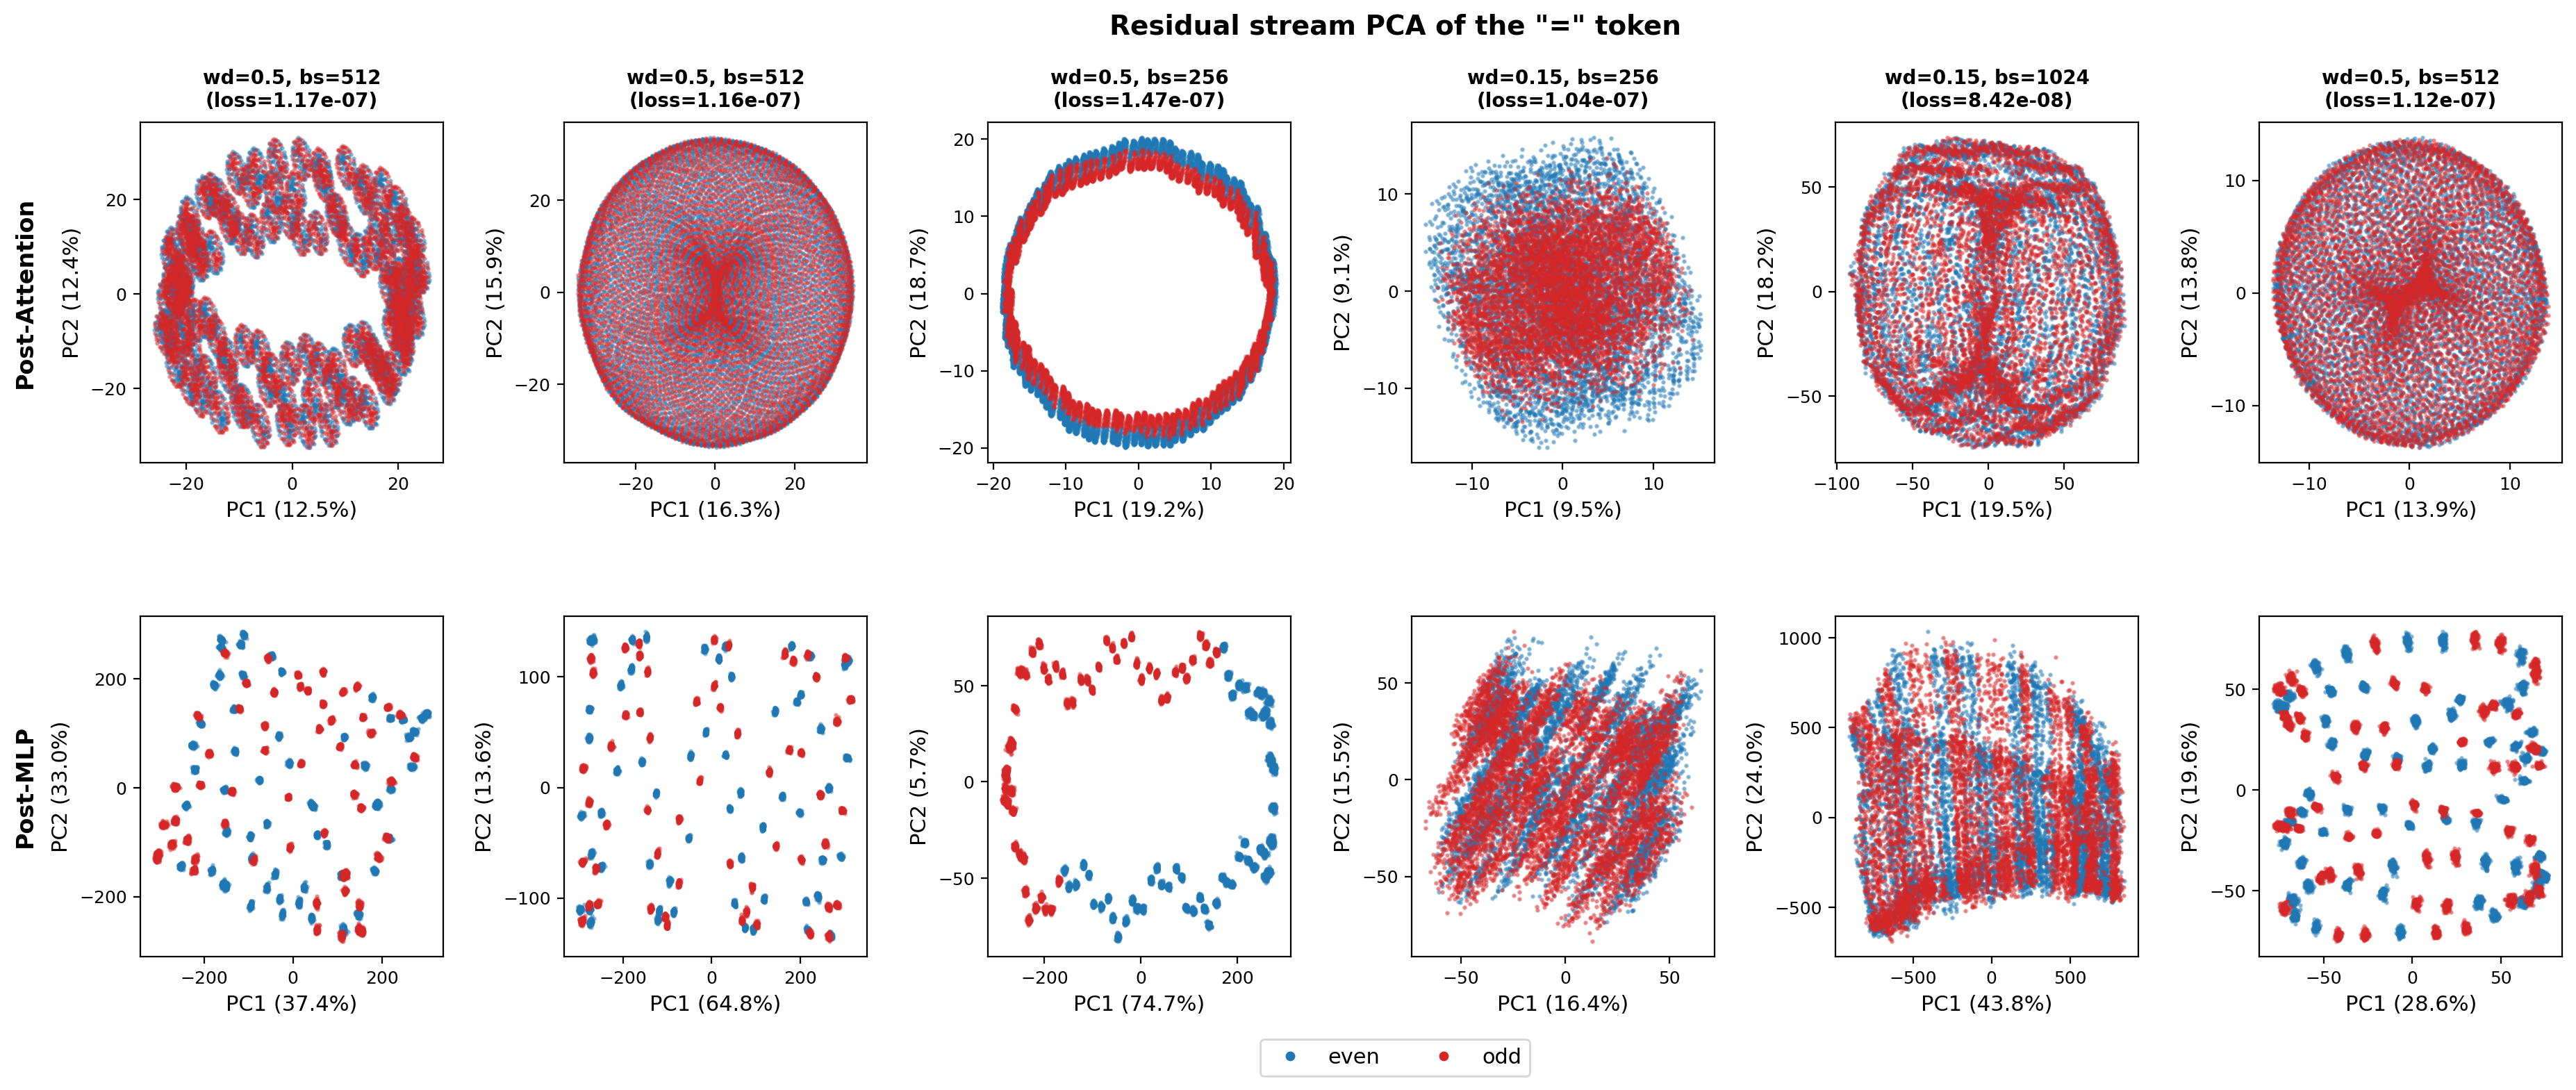
\includegraphics[width=0.9\textwidth]{figs/pca_top_pt.png}
    \caption{\PT{}}
    \label{fig:pca_top_pt}
  \end{subfigure}\\[1em]
  \begin{subfigure}{\textwidth}
    \centering
    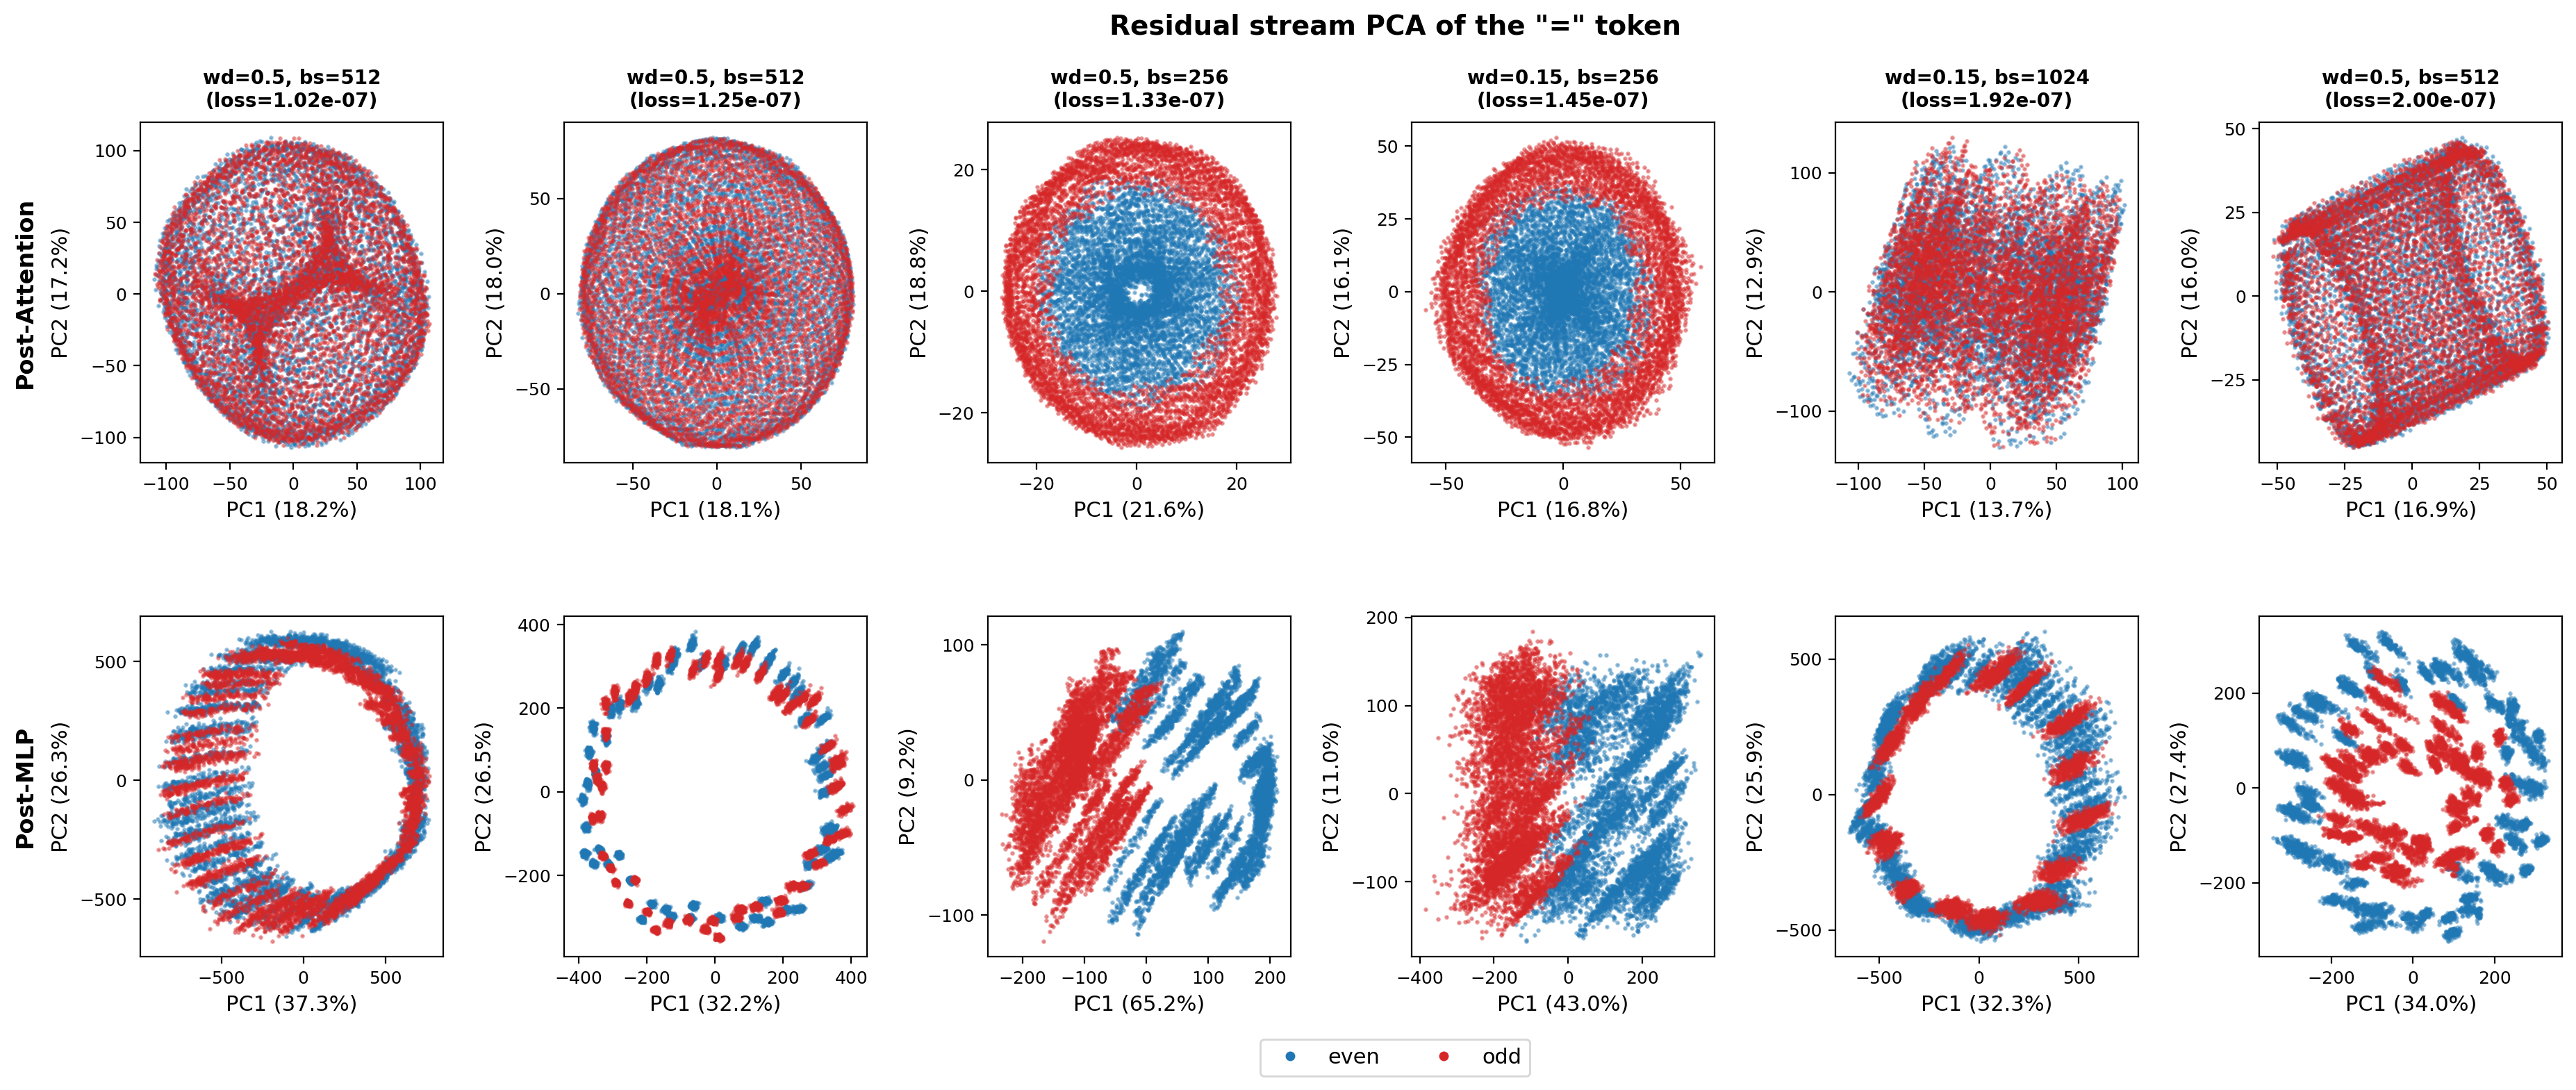
\includegraphics[width=0.9\textwidth]{figs/pca_top_sft.png}
    \caption{\POST{}}
    \label{fig:pca_top_sft}
  \end{subfigure}\\[1em]
  \begin{subfigure}{\textwidth}
    \centering
    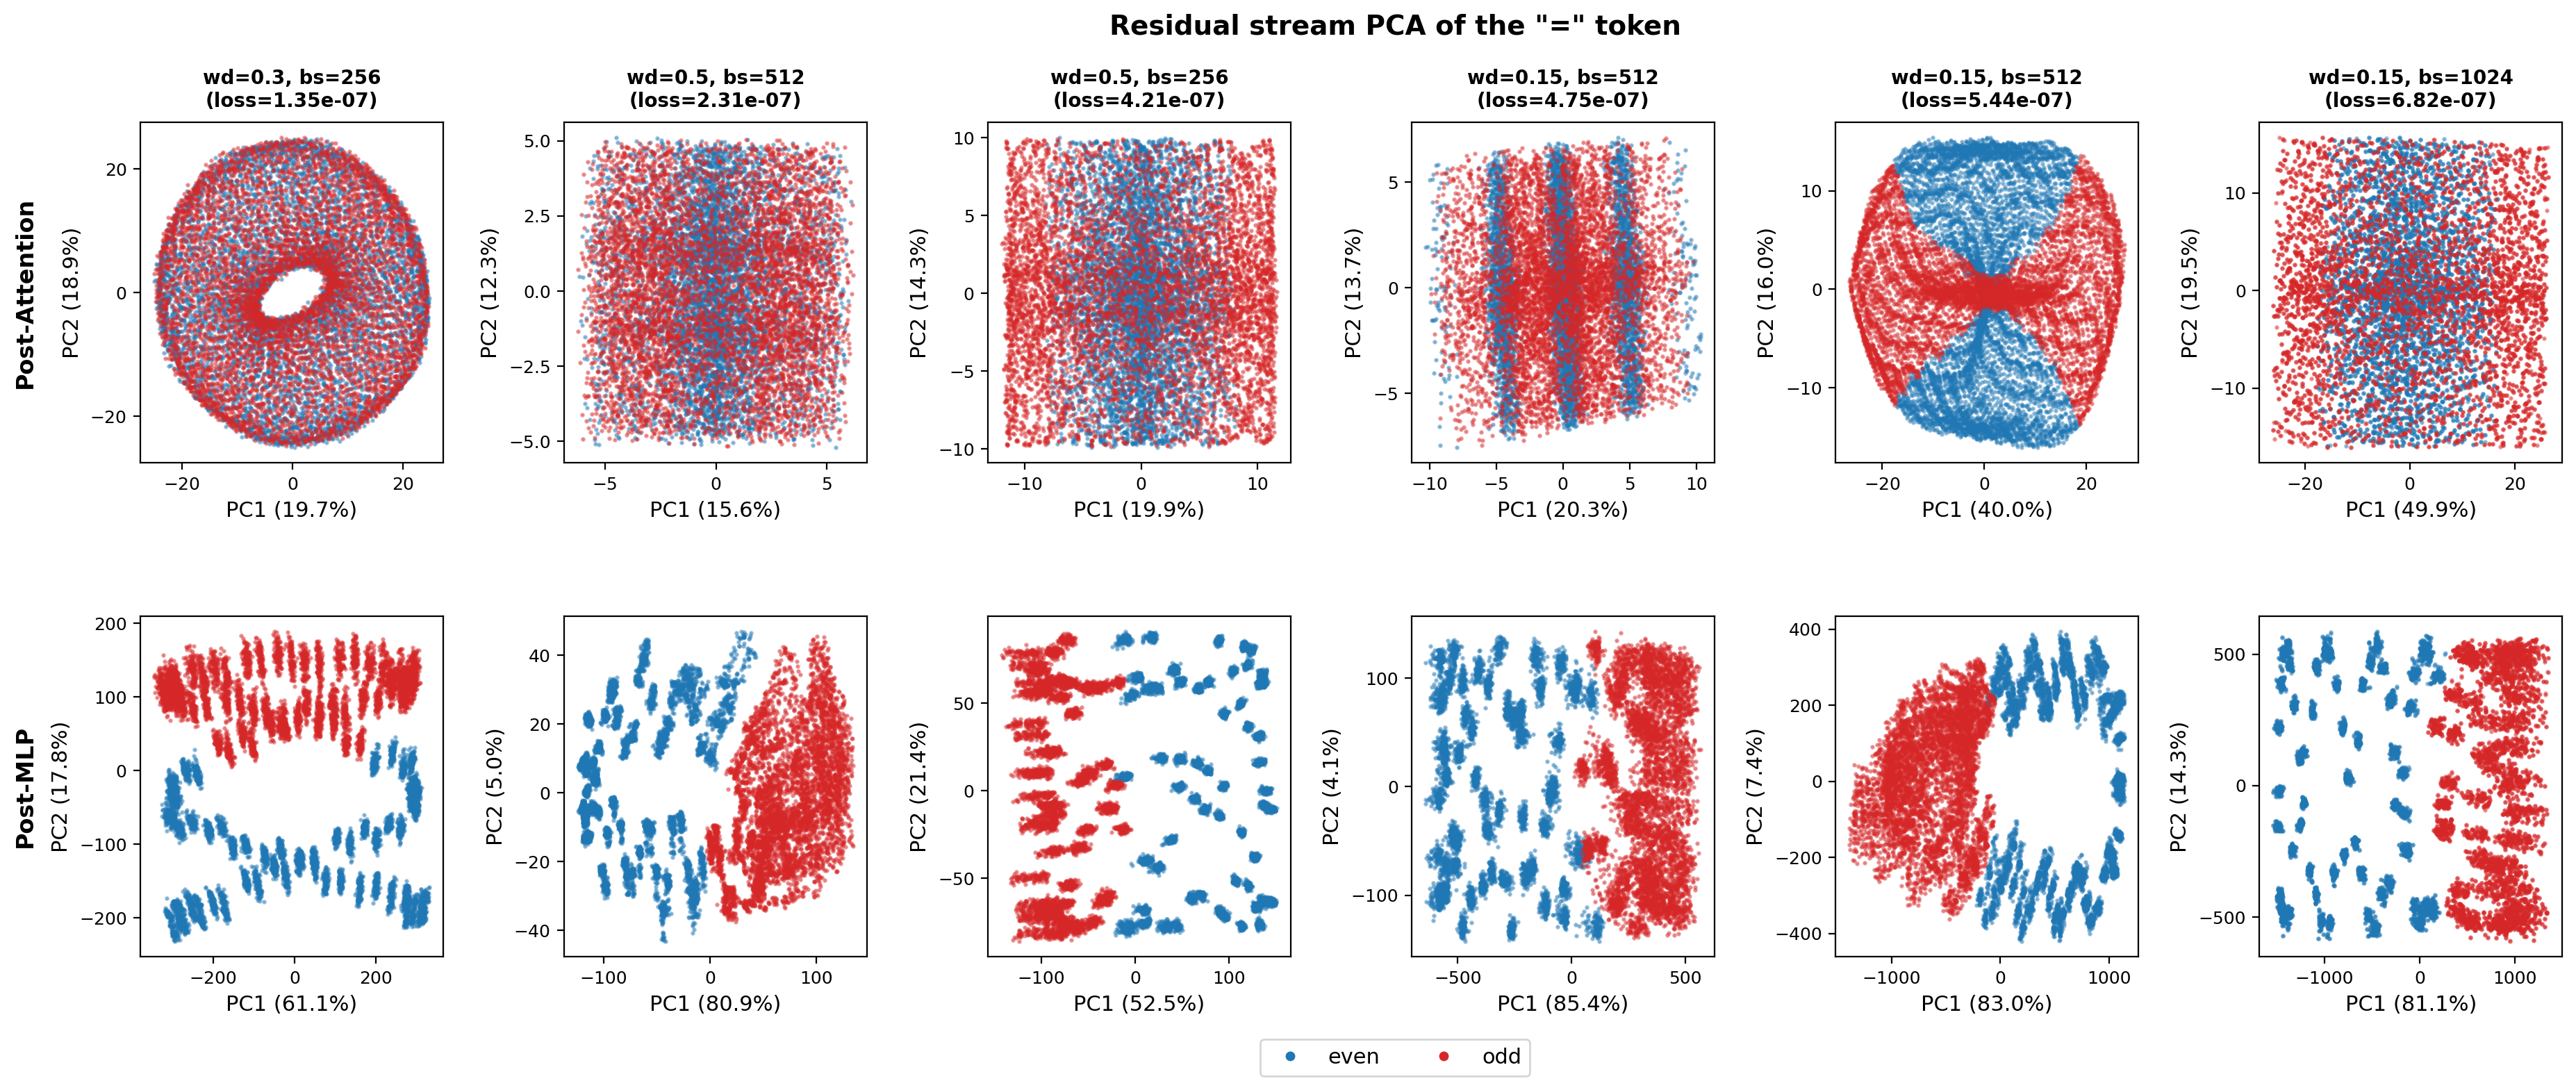
\includegraphics[width=0.9\textwidth]{figs/pca_top_ptg.png}
    \caption{\PTG{}}
    \label{fig:pca_top_ptg}
  \end{subfigure}
  \caption{Residual stream PCA for the six best models of each variant. \POST{} and \PTG{} are sorted by their own test loss; \PT{} is sorted by the corresponding \POST{} test loss to enable direct comparison of matched model pairs. Even/odd coloring reflects result parity.}
  \label{fig:pca_sweep}
\end{figure}

Although the main text presents PCA projections from a single canonical model per variant, the qualitative structure of these projections is not identical across hyperparameter and seed choices.
\Cref{fig:pca_sweep} shows the residual stream PCA of the \texttt{=} token for the six lowest test loss models of each variant.
Despite all achieving near-perfect accuracy, the PCA projections differ noticeably---reflecting differences in the learned representations that are not captured by aggregate metrics alone.

\end{document}
